%%%%%%%%%%%%%%%%%%%%%%%%%%%%%%%%%%%%%%%%%%%%%%%%%%%
%
%  New template code for TAMU Theses and Dissertations starting Fall 2012.  
%  For more info about this template or the 
%  TAMU LaTeX User's Group, see http://www.howdy.me/.
%
%  Author: Wendy Lynn Turner 
%	 Version 1.0 
%  Last updated 8/5/2012
%
%%%%%%%%%%%%%%%%%%%%%%%%%%%%%%%%%%%%%%%%%%%%%%%%%%%
%%%%%%%%%%%%%%%%%%%%%%%%%%%%%%%%%%%%%%%%%%%%%%%%%%%%%%%%%%%%%%%%%%%%%%
%%                           SECTION III
%%%%%%%%%%%%%%%%%%%%%%%%%%%%%%%%%%%%%%%%%%%%%%%%%%%%%%%%%%%%%%%%%%%%%

\chapter{\uppercase{Related work}}
There are so many research scientists working in large oil \& gas companies and so many service companies, but in such a mature industry, it is very difficult to find complete open source codes or sample data on Internet. The main reason should be Intellectual Property issue; In the last twenty years, the oil \& gas becomes the most profitable industry. As there are less unexplored areas, how to find the valuable oilfield is the most important task for oil \& gas companies. With the intensifying competition, the exploration data became very expensive and every company either kept its technology secret or applied for patents to protect itself.    

In normal case of seismic data processing, most companies will both write their own algorithms and use commerical softwares such as MATLAB, Petrel from Schlumberger, Paradigm software suite etc. The previous ones are mostly used to verify and its own customized algorithms or models and could be optimized basing on requirement, on the other hand, commercial softwares are mainly used in migration and interpretation stages. As for the commerical softwares, most of them could only run on single node, the performance is critical problem while handling big data.  
Besides commerical softwares, there is a list of free geophysics software in \cite{listofgeosw}. Among them the most famous one is Seismic Unix (SU) \cite{SUHome}. SU provides a series of tools for seismic data processing, such as data loading and storing data to and from files, data format conversion, transformation and filtering, processing utilities including stacking data, velocity analysis and migration etc.\cite{SUManual}. SEPlib \cite{SEPlibHome} contains programs to manipulate and process many types of geophysical data. It introduces two principles: Separate the geometry information from the seismic data, and exploit as much as possible the existing regularity in the data geometry, thus enable users and programmers to deal with irregularly sampled data with the same simplicity and efficiency \cite{SEPManual}. Madagascar \cite{MadagascarHome} is a moden package that provide a powerful for multidimensional data analysis and reproducible computational experiments. It provides two main ways of running application: shell scripts that use piping mode to run programm similiar to seismic unix, and Python scripts using SCons. Comparing with SU, Madagascar provide more programms and an open platform that support multi-language (C,Python and Fortran 90) on which user could add his own programms and share with others. The Mines Java Toolkit (JTK) \cite{JTKHome} is a set of Java packages and native (non-Java) code libraries for science and engineering including digital signal processing and 2-D and 3-D graphics. OpenSeaSeis \cite{OpenSeaSeis} is a sequential trace flow system, following the same basic concept of most other existing seismic processing systems that are using standard I\/O for passing traces from module to module as SU or have a base system for managing the trace flow.





Text goes here \cite{ApacheHadoop}. 


\section{Apache Hadoop}

%%%%%%%%%%%%%%%%%%%%%%%%%%%%%%%%%%%%%%%%%%%%%%%%%%%%%%
\begin{figure}[H]
\centering
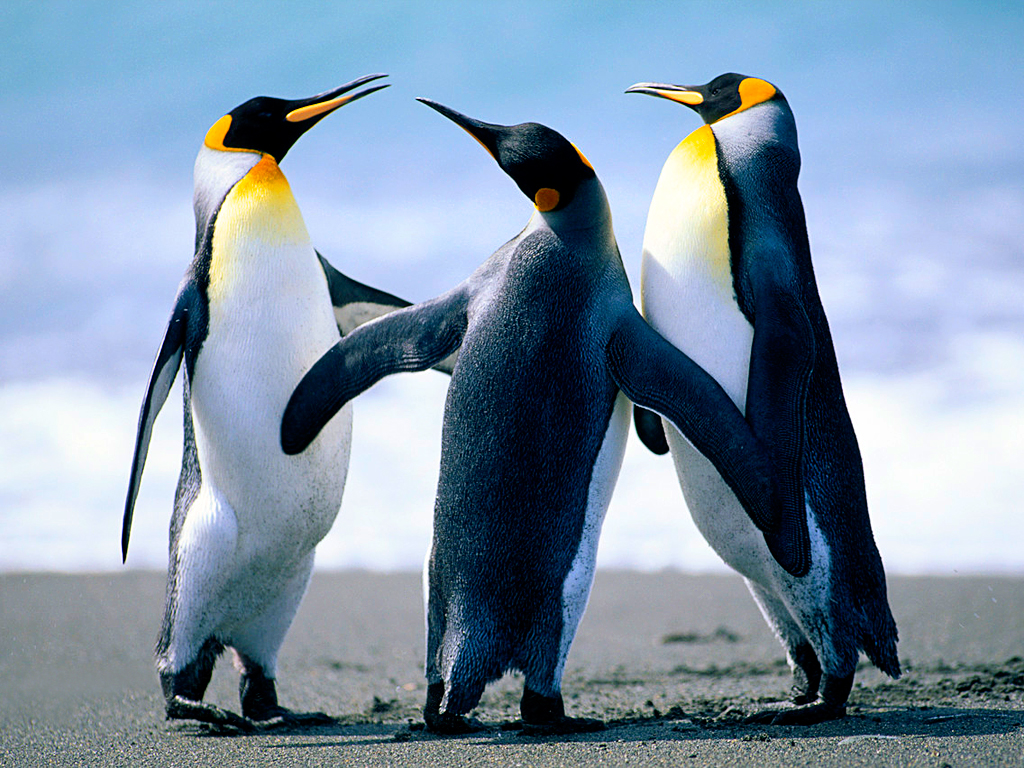
\includegraphics[scale=.50]{figures/Penguins.jpg}
\caption{TAMU figure}
\label{fig:tamu-fig3}
\end{figure}
%%%%%%%%%%%%%%%%%%%%%%%%%%%%%%%%%%%%%%%%%%%%%%%%%%%%%%
\section{Apache Spark}

Text between the figures.  Text between the figures. Text between the figures. Text between the figures.  Text between the figures. Text between the figures. Text between the figures.  Text between the figures. Text between the figures. Text between the figures.  Text between the figures. Text between the figures.
%%%%%%%%%%%%%%%%%%%%%%%%%%%%%%%%%%%%%%%%%%%%%%%%%%%%%%%
%\begin{figure}[H]
%\centering
%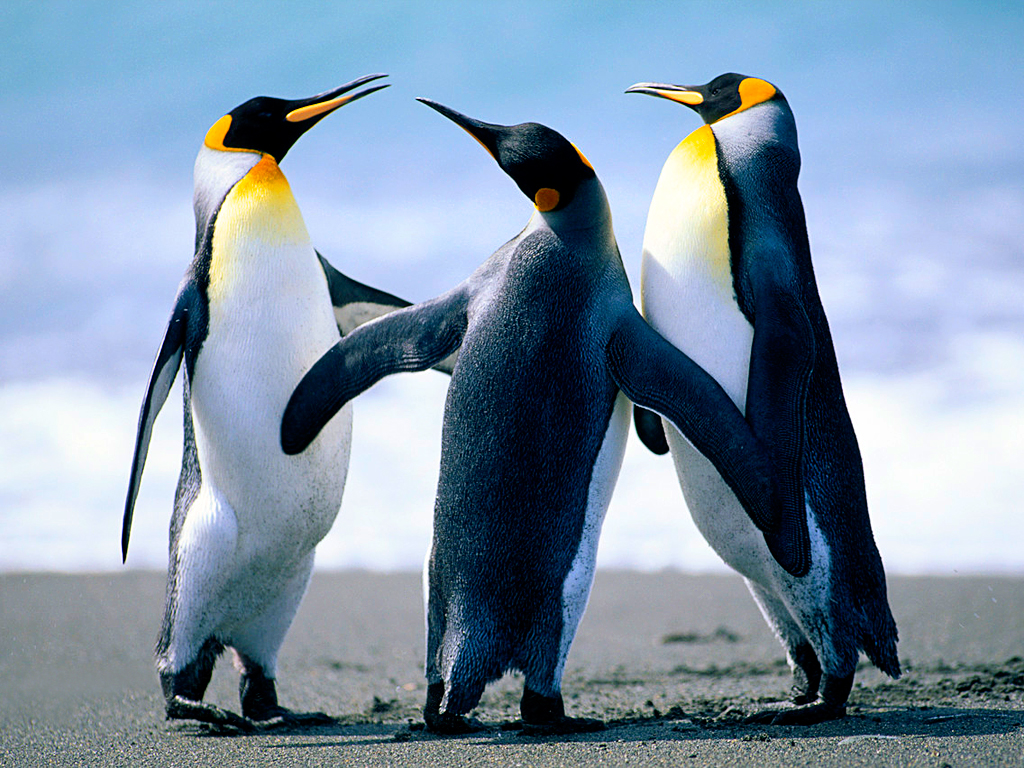
\includegraphics[scale=.50]{figures/Penguins.jpg}
%\caption{Another TAMU figure}
%\label{fig:tamu-fig4}
%\end{figure}
%%%%%%%%%%%%%%%%%%%%%%%%%%%%%%%%%%%%%%%%%%%%%%%%%%%%%%%

\subsection{Subsection}

%%%%%%%%%%%%%%%%%%%%%%%%%%%%%%%%%%%%%%%%%%%%%%%%%%%%%%%
%\begin{figure}[H]
%\centering
%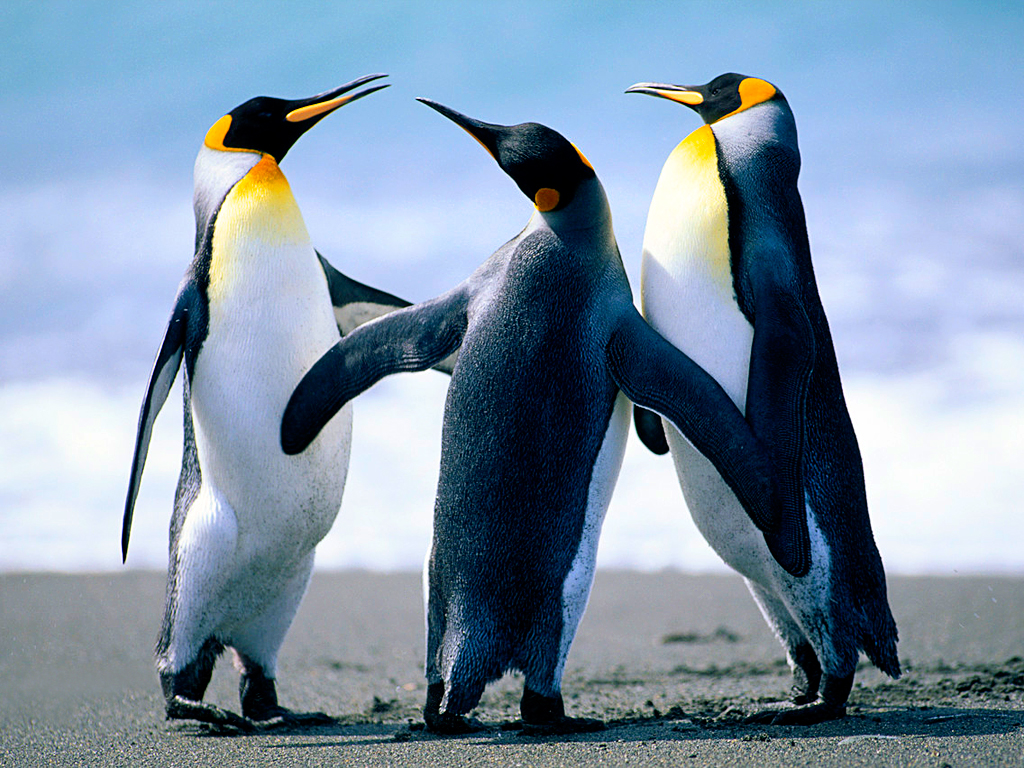
\includegraphics[scale=.50]{figures/Penguins.jpg}
%\caption{Another TAMU figure}
%\label{fig:tamu-fig4-2}
%\end{figure}
%%%%%%%%%%%%%%%%%%%%%%%%%%%%%%%%%%%%%%%%%%%%%%%%%%%%%%%
\subsection{Subsection}

A table example is going to follow.

\begin{table}[H]
\centering
\caption{This is a table template}
\begin{tabular}{|l|c|c|c|c|c|}
\hline
Product & 1 & 2 & 3 & 4 & 5\\
\hline
Price & 124.- & 136.- & 85.- & 156.- & 23.-\\
Guarantee [years] & 1 & 2 & - & 3 & 1\\
Rating & 89\% & 84\% & 51\% & & 45\%\\
\hline
\hline
Recommended & yes & yes & no & no & no\\
\hline
\end{tabular}
\label{tab:template2}
\end{table}
\subsubsection{This is a subsubsection}

\section{Python}



